
\section{Single Agent Approach}

The goal of this section was to design a system that fulfilled the requirements outlined in Problem~\ref{prob:sub2}

The general shape of a GA as seen in Algorithm~\ref{alg:GenericGA} is the same for almost all problems. But each individual operator implementation is domain specific.

\subsection{Individual Encoding}
As such, I first had to implement a method to generate an initial population. In order to do this, I had to define my programmatic representations of the phenotypes and genotypes of my individuals. I decided to base my genotypic structure on the that described by Kala\cite{kalaOnroadIntelligentVehicles2016}.

In this approach, the genotype is abstractly represented as a Bézier curve (Section~\ref{sec:back-bezier-curves}). This is more concretely translated into a real-valued string, interleaving the $x$ and $y$ coordinates of each control point. Taking the form:

\begin{figure}[ht]
	\centering
	\begin{tikzpicture}[
			block/.style={minimum height=2.2em,outer sep=0pt,draw,rectangle,node distance=0pt}]

		\node [block] (A) {$P_{0_{x}}$};
		\node [block, right = of A] (B) {$P_{0_{y}}$};
		\node [block, right = of B] (C) {$P_{1_{x}}$};
		\node [block, right = of C] (D) {$P_{1_{y}}$};
		\node [block, right = of D] (E) {$\ldots$};
		\node [block, right = of E] (F) {$P_{n_{x}}$};
		\node [block, right = of F] (G) {$P_{n_{y}}$};

	\end{tikzpicture}
	\caption{\label{fig:GA_Genotype} Individual genotype as real-valued string }
\end{figure}

In the above form the descriptions of genetic operators found in Section~\ref{subsec:GAOps} should be sufficiently detailed to re-implement.\todo{Phrasing?  Correct? should I elaborate?}

Initially my Phenotype contained no additional information. However, I still created the distinction to allow for additional properties to be encapsulated during development.

\subsection{Population Generation}

Population generation theoretically can be very simple and generate very little diversity, relying on the other operators to explore the search space. However, the more diverse a set of initial routes one can generate, the quicker the system will converge to an optimal solution.

As such we want to ensure that both the number of control points as well as their position are properly varied.

The first and last control points \textbf{must} be the starting and goal position for the agent. In a Bézier curve these are the only two points that the curve definitely passes through. We must also ensure that the $x$ coordinates of the control points are in order, so as to avoid routes which \textit{double back} on themselves. This can also occur as the result of other operators such as crossover and mutation, we can fix this using a simple repair operator which re-orders points based on their $x$ positions.


\subsection{Fitness assessment}

The foundation of my Fitness function is the length of each route, i.e. the length of a given $n$ degree Bézier curve. This calculation can be accurately approximated using Equation~\ref{eq:bezlength} as the true calculation is expensive and does not generalise nicely to $n$ degrees\cite{gravesenAdaptiveSubdivisionLength1997}.

Minimising the length of a route is a good way of ensuring generated routes are direct, however, other values and heuristics are required to maintain other requirements such as to make sure changes in direction are not too severe or that a route does not pass through infeasible space (avoiding obstacles etc.).

I initially experimented with an alternative coordinate space which enabled me to completely enclose the search space within the area of the road, eliminating the possibility of generating routes that left the \textit{road}. This was inspired by the ``Road coordinate axis system'' described by Kala in~\cite{kalaOptimizationBasedPlanning2016}. However I abandoned this concept as it did not appear to increase performance and introduced overhead when visualising or generating the routes.

Instead I defined each section of road using the following Structure:

\begin{minted}{julia}
struct Road
    boundary_1::Function
    boundary_2::Function
    obstacles::Array{Obstacle}
    length::Real
end
\end{minted}

This approach allows me to define the upper and lower boundary of a road as any function, straight roads can be defined as a pair of straight lines a certain width apart, and arbitrarily complex roads can be represented using arbitrarily complicated functions.

For example the road seen in Figure~\ref{fig:simple-road} had boundary functions:

\begin{align*}
  b_{1}(x) &= 0 \\
  b_{2}(x) &= 5
\end{align*}

And the curved road section seen in Figure~\ref{fig:curved-road} functions:

\begin{align*}
  b_{1}(x) &= 2\cosh (0.1x)-2 \\
  b_{2}(x) &= 2\cosh(0.12x)+8
\end{align*}

Where in both cases the length of the road (and therefore upper bound of $x$) was 25, the lower bound of $x$ was 0.

\begin{figure}[ht]
  \centering
  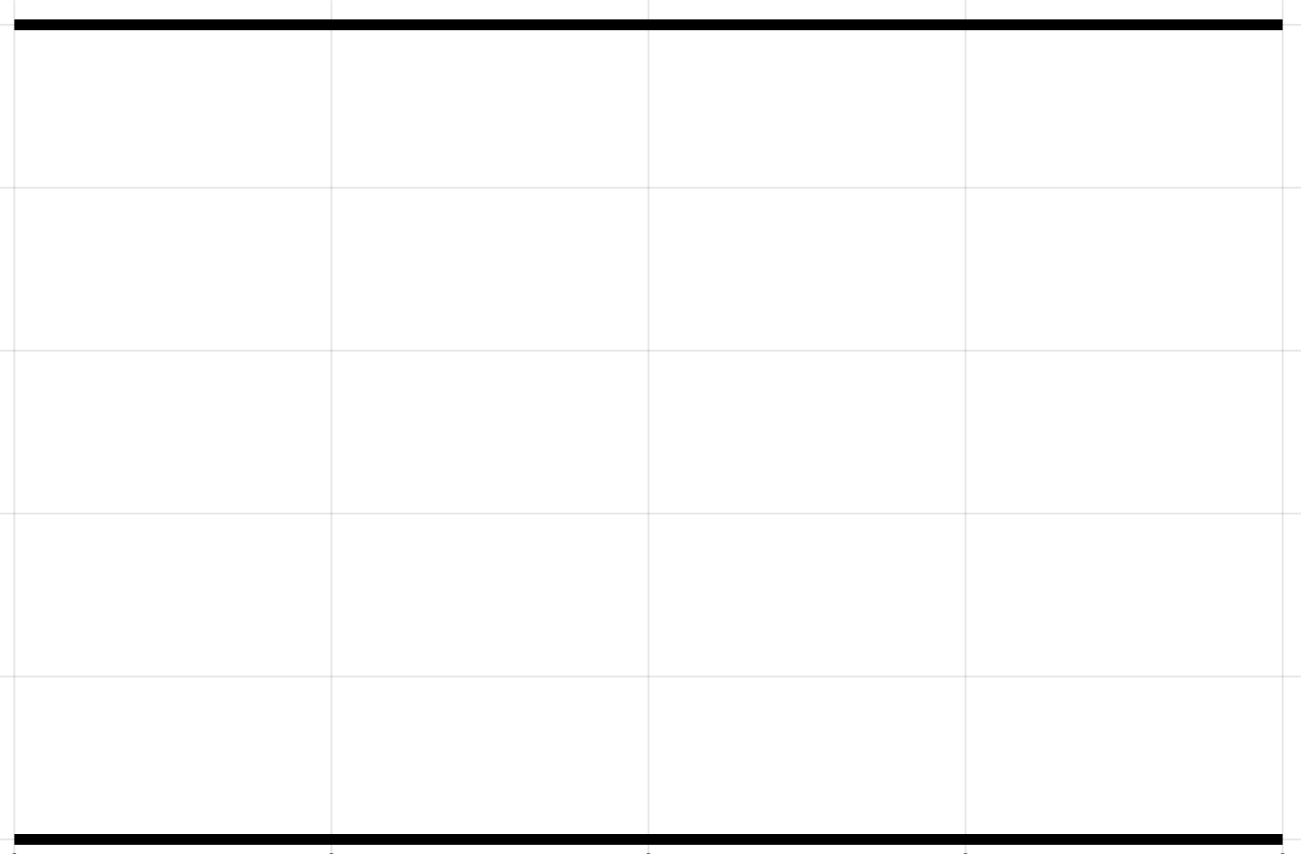
\includegraphics[scale=0.2]{figures/simple-road.png}
  \caption{\label{fig:simple-road} A straight road}
\end{figure}

\begin{figure}[ht]
  \centering
  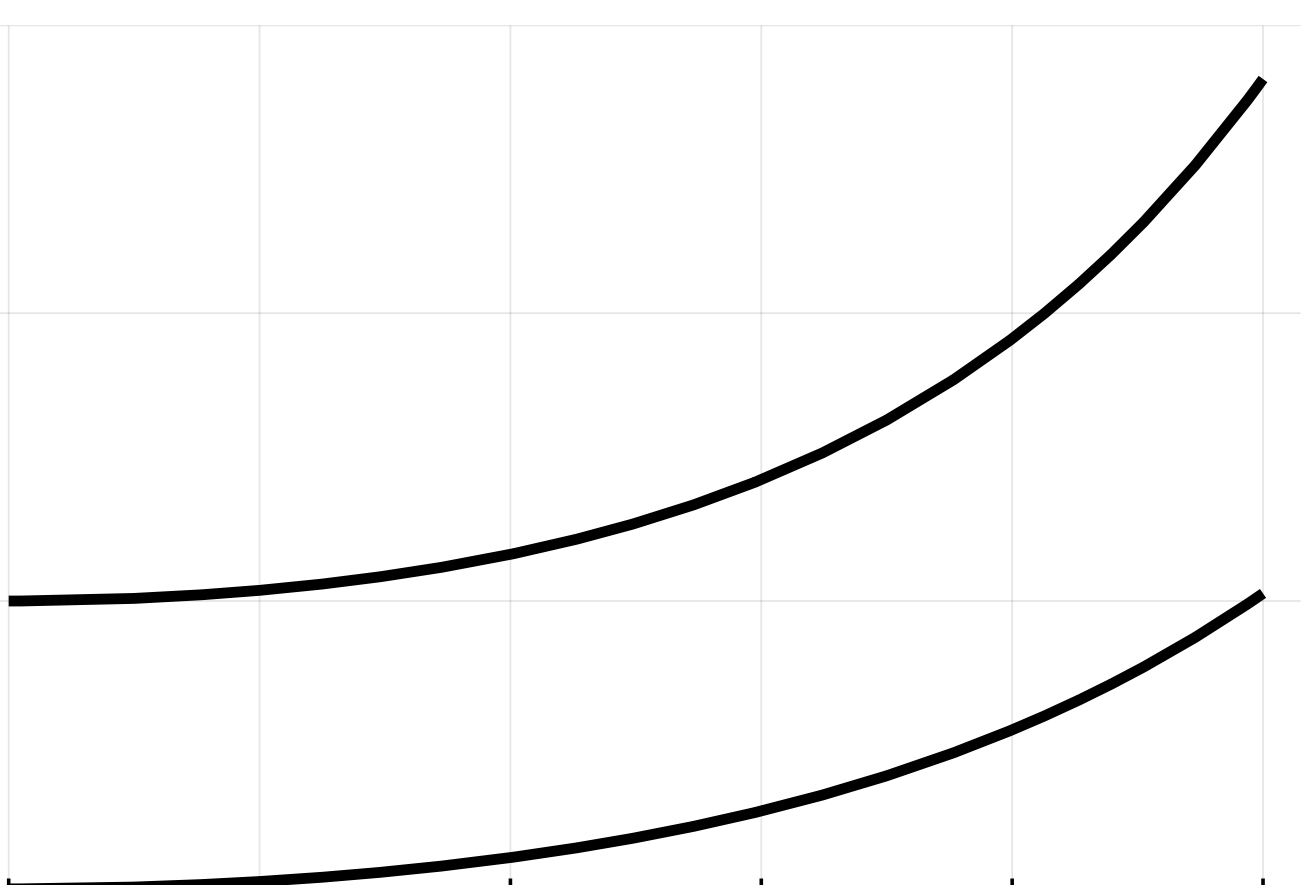
\includegraphics[scale=0.2]{figures/curved-road.png}
  \caption{\label{fig:curved-road} A curved road}
\end{figure}

\paragraph{Road Obstacles}

I have implemented two basic \texttt{Obstacle} types (\texttt{Rectangle} and \texttt{Circle}) allowing me to create regions of infeasible space within the valid road-space.

Infeasible space is then calculated by taking a sample of 500 points along a given curve $B$ and checking which (if any) lie within any of the obstacles.

A Bézier curve is then constructed using two applications of De Casteljau's algorithm (See Section~\ref{sec:decasteljau}) using values for $t$ derived from the subsample points. An illustration of this process can be seen in Figure~\ref{fig:ifspace-illustration}. The length of this curve is weighted and added to the overall fitness of the candidate solution. The stages progress as Follows:

\begin{enumerate}
  \item Curve and obstacle drawn
  \item Uniform sample of points chosen along curve
  \item Curve segment from origin to first infeasible point isolated
  \item Curve segment from last infeasible point to end position isolated
  \item Infeasible distance calculated as difference in length between original curve and two isolated segments
\end{enumerate}


A similar process is performed to determine how much of a curve passes too closely to an infeasible region, this is penalised with a separate, lower, weighting.

\begin{figure}
  \centering
  \begin{subfigure}[b]{0.44\textwidth}
    \centering
    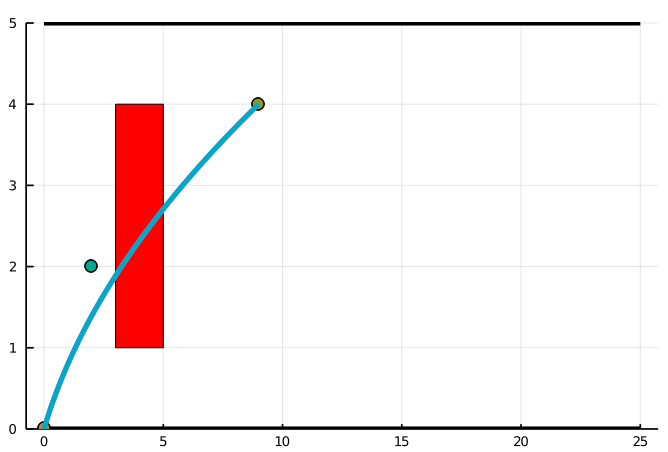
\includegraphics[width=\textwidth]{figures/obstacleavoidance-stage1.png}
    \caption{Stage 1}
  \end{subfigure}
  \begin{subfigure}[b]{0.44\textwidth}
    \centering
    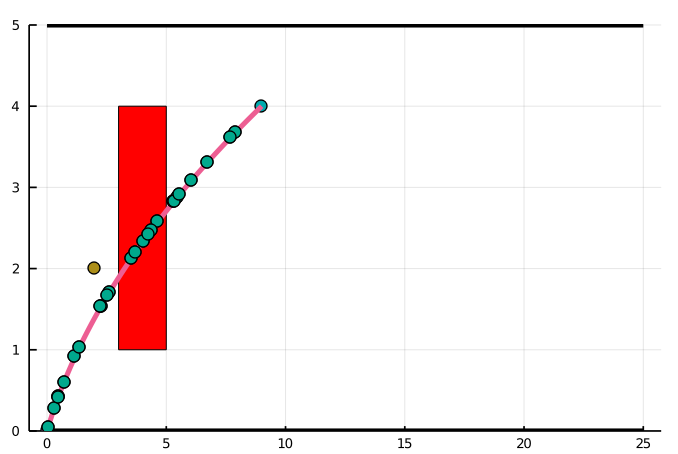
\includegraphics[width=\textwidth]{figures/obstacleavoidance-stage2.png}
    \caption{Stage 2}
  \end{subfigure}
  \begin{subfigure}[b]{0.44\textwidth}
    \centering
    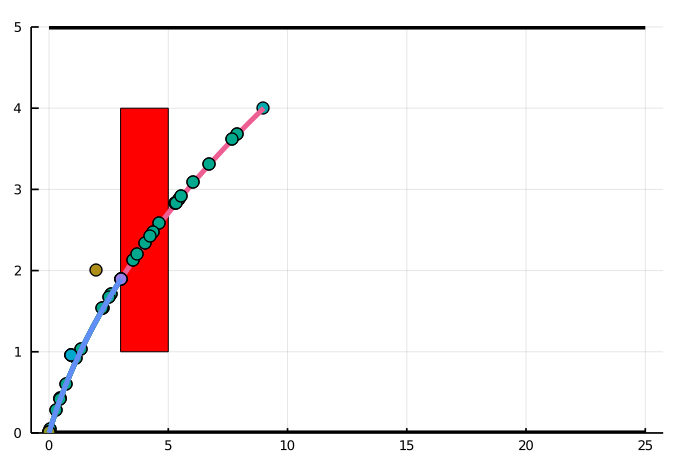
\includegraphics[width=\textwidth]{figures/obstacleavoidance-stage3.png}
    \caption{Stage 3}
  \end{subfigure}
  \begin{subfigure}[b]{0.44\textwidth}
    \centering
    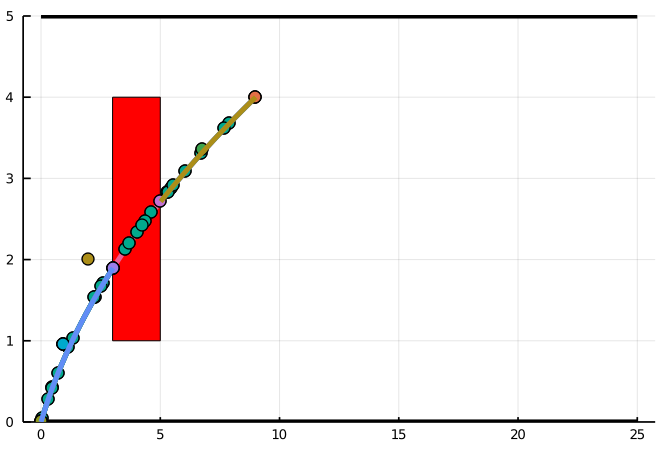
\includegraphics[width=\textwidth]{figures/obstacleavoidance-stage4.png}
    \caption{Stage 4}
  \end{subfigure}
  \begin{subfigure}[b]{0.44\textwidth}
    \centering
    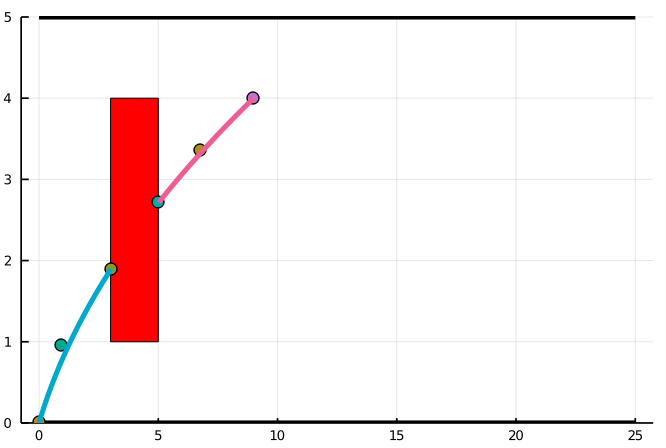
\includegraphics[width=\textwidth]{figures/obstacleavoidance-stage4-aux.png}
    \caption{Stage 5}
  \end{subfigure}
  \caption{\label{fig:ifspace-illustration} Illustration of finding infeasible section of curve}
\end{figure}\todo{Remove hand-drawn figure and move descriptions to paragraph instead of caption}

Once the initial population is generated, the main algorithmic loop can begin, this is the repeated application of the selection, crossover, mutation and evaluation operators (See Section~\ref{subsec:GAOps}) until set termination criteria are met or the maximum number of generations is completed, seen in Algorithm~\ref{alg:GenericGA}.

The final set of routes is finally filtered by the predicate $\texttt{infeasible-distance}(i) = 0 $

\section{Multi-agent Approach}

So far we have only concerned ourselves with planning a route through a road-space for a single agent. However, in the real world, roads are seldom occupied by a single vehicle and as such we must consider how to efficiently plan a set of routes for a set of agents between between a set of coordinate pairs, such that, our agents do not collide at any point in time.

There are different approaches we can take to this problem. \todo[inline]{refer to lit rev sections discussing approaches by Kala\cite{kalaOnroadIntelligentVehicles2016} and Cai \& Peng \cite{caiCooperativeCoevolutionaryAdaptive2002}}

My initial approach to a collaborative planning system was somewhat inefficient. The system operated by planning routes for each agent sequentially, using a growing \textit{context} to keep track of the routes that had already been finalised. The first agent to be planned was not concerned with avoiding collisions, as, as far as it was concerned, there were no other agents in the system. Each subsequent agent checked if any of its candidate solutions intersected with and of the routes planned before, a very high penalty was applied to any routes with collisions.

This system was very inefficient with the final routes requiring a large number of checks to be carried out by my \texttt{bezInt} function, which itself suffered from \todo[inline]{verify this} exponential time (and space) complexity.

This system was improved upon by splitting the process over multiple threads, each agent being given a separate thread, communicating their most up-to-date plans via a shared array, $S$. Agent $i$ will store its current fittest route in $S[i]$, the fitness of any candidate checks for collisions with each route in $S$. This system may conduct more checks but it removes the problem of prioritising the first route to the planned and reduces the overall runtime of the system approximately proportionally to the number of threads available.

\subsection{Collision Detection}
\label{subsec:col-detection}

Collision detection is one of the core obstacles to a viable cooperative route planner. You must be able to certify that your resulting set of routes do not collide at any point in time, else the entire system fails.

Simply detecting intersections is not enough as two routes can intersect but only collide if they pass through the same point at the same time. We therefore require some notion of time when realising our Bézier curve routes.

I made the assumption that each agent in my system travels at a uniform constant speed. To remove this assumption we would need to include a velocity-time profile in the genotype of each individual, this is an area for further research.

With this assumption, we can now say that two routes collide if they intersect and the distance from their respective origins and the point of intersection is the same. We have now reduced this problem to finding a point of intersection between two Bézier curves, this is still a non-trivial task.

\subsubsection{Bézier Curve intersection}

The commonly employed technique for finding intersections between two $n$-degree Bézier curves is repeated recursive subdivision. Whilst it is possible to precisely calculate the point of intersection it is very difficult and computationally expensive and does not generalise well to $n$ degrees. For example, to numerically find the intersection two curves of degree 3 we must solve a $9^{th}$ order equation, producing unstable results. This is described by Bézout's theorem which states that two planar algebraic curves of degrees $d_{1}$ and $d_{2}$ will have up to $d_{1}d_{2}$ intersection points.\todo{cite this or remove it}

In their 2006 paper Yap\cite{yapCompleteSubdivisionAlgorithms2006} proposed an efficient method for finding the intersection of two Bézier curves through a 2 stage process surrounding repeated subdivision.

During development I attempted to use a Bézier curve library (\texttt{libbezier})\cite{Hermes2017} written for python but featuring a core written in Fortran, providing a C ABI. Julia, featuring interoperability with C and Fortran, allowed me to make direct calls to the Fortran subroutines and C functions. Ultimately, however, I encountered too many issues stemming from this library's inability to be run in parallel along with seemingly random segfaults which I struggled to diagnose through two levels of language abstraction (Fortran $\rightarrow$ C $\rightarrow$ Julia); this led me to write my own functions natively in Julia, although replicating the same accuracy as the nearly 4000 lines of Fortran proved challenging.

In order to speedup my Bézier intersection function I implemented a number of time saving measures:

\begin{enumerate}
  \item If the convex hulls of two curves $B_{1}$ and $B_{2}$ intersect, i.e. some amount of the area of the convex hull of $B_{1}$ ($CH(B_{1})$), lies inside the convex hull of $B_{2}$ ($CH(B_{2})$) then there may  be some intersection and as such, further checks are required. If however, this is not the case then (likely) the two curves do not intersect and the function can exit early.

        This is a simplified version of the logic presented by Yap in his \textit{Micro Phase} of intersection detection. However, in order to cover all edge cases and make this a reliable rule to follow a lot more precomputation is required (See Elementary curves \& curve coupling in~\cite{yapCompleteSubdivisionAlgorithms2006}).

        As such, I ended up removing this feature as the additional work required was too high for this project.\todo{phrasing? }
    \item I instead instituted a simpler heuristic using bounded boxes (See Section~\ref{subsec:back_boundedboxes}). Using the \texttt{Luxor} library \todo{cite?} I was able to detect whether two bounded boxes intersected, if they did not, further checks can be skipped.\todo{Merge these first 2? }
  \item If two curve segments have already been checked for intersection, why bother checking them again?

        This question was solved by trading computation time for memory, by constructing a hash table linking curve pairs to a tuple of intersection curve segments (if present) and a boolean, when checking two curve sections, if they already exist in the hash table the remaining computation can be skipped with the precomputed result returned instead.

        In most cases a check is performed at least twice. Given two candidate solutions for two distinct agents $B_{1}$ and $B_{2}$, when evaluating the fitness of $B_{1}$ it is checked for intersections with $B_{2}$ and equally when evaluating the fitness of $B_{2}$ $B_{2}$ is checked against $B_{1}$, thus buy storing the first result, the second check can be skipped.

        In reality, many curve segments are found repeatedly inside of populations and as such many more duplicate checks can be skipped through this method.
  \item I implemented a recursion depth limit so as to introduce an upper bound in computation before the function returns false. Without this I found that often the checks would repeat until it was searching for intersections between infinitesimally small curve sections.

  \item I was also able to reduce the runtime of this function via the use of threading. Upon a subdivision two more threaded tasks are spawned and the disjunction of their results returned. The optimal case for this approach is that the intersection occurs early on in the curve as the task results must be fetched sequentially in the order that they were spawned. \todo{remove this sentence?}

\end{enumerate}




\section{Language Choice}\todo[inline]{decide whether to remove this, I am thinking yes but last para is interesting, maybe move to evaluation}

I have chosen to implement my approach using the Julia language project\cite{JuliaProgrammingLanguage}.

Julia is a relatively new language first developed in 2012 by Jeff Bezanson, Stefan Karpinski and Viral Shah. It is a multi-paradigm language allowing for functional, object oriented and meta programming approaches to problems. I will mainly be using it for it's functional and OO capabilities.

Julia operates using multiple dispatch similar to languages such as Haskell. It interoperates with C and Fortran codebases without the need of middle-man bloat. This fact allows it to utilise the extensive high performance C libraries for floating point operations. Julia is eagerly evaluated, uses a Just in time compiler and has a garbage collector.

Julia features a syntax similar to both Python and Matlab with performance on par with C. As I am already very familiar with python and have studied functional programming in a number of modules; I found this language very quick and intuitive to learn and the resulting code to be clean, idiomatic and fast.

A real-world deployment of a system based on my research would undoubtedly be required to run on small, relatively low performance, embedded systems and as such Julia may not be appropriate here. A language such as C or Rust may be used instead.

Julia also has distributed computation facilities. This sort of functionality could be extremely useful in a system such as mine as it could allow for computation to be spread across the agents themselves, removing the need for a central planning centre which could be a single point of failure.


\section{Results}

Due to the high dimensionality of my search space, I cannot visualise the objective function of my GA.

My results were achieved by 

%TC:macro \todo 1

%%% Local Variables:
%%% mode: latex
%%% TeX-master: "report"
%%% End:
